% Created by tikzDevice version 0.12.3.2 on 2022-02-15 18:25:40
% !TEX encoding = UTF-8 Unicode
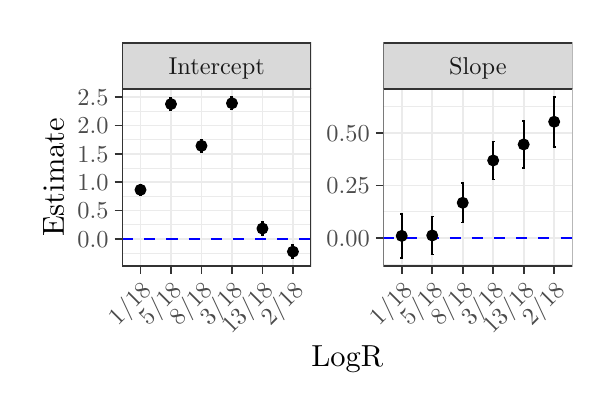
\begin{tikzpicture}[x=1pt,y=1pt]
\definecolor{fillColor}{RGB}{255,255,255}
\path[use as bounding box,fill=fillColor,fill opacity=0.00] (0,0) rectangle (202.36,130.09);
\begin{scope}
\path[clip] (  0.00,  0.00) rectangle (202.36,130.09);
\definecolor{drawColor}{RGB}{255,255,255}
\definecolor{fillColor}{RGB}{255,255,255}

\path[draw=drawColor,line width= 0.6pt,line join=round,line cap=round,fill=fillColor] ( -0.00,  0.00) rectangle (202.36,130.09);
\end{scope}
\begin{scope}
\path[clip] ( 34.16, 43.96) rectangle (102.46,108.01);
\definecolor{fillColor}{RGB}{255,255,255}

\path[fill=fillColor] ( 34.16, 43.96) rectangle (102.46,108.01);
\definecolor{drawColor}{gray}{0.92}

\path[draw=drawColor,line width= 0.3pt,line join=round] ( 34.16, 48.62) --
	(102.46, 48.62);

\path[draw=drawColor,line width= 0.3pt,line join=round] ( 34.16, 58.88) --
	(102.46, 58.88);

\path[draw=drawColor,line width= 0.3pt,line join=round] ( 34.16, 69.14) --
	(102.46, 69.14);

\path[draw=drawColor,line width= 0.3pt,line join=round] ( 34.16, 79.40) --
	(102.46, 79.40);

\path[draw=drawColor,line width= 0.3pt,line join=round] ( 34.16, 89.65) --
	(102.46, 89.65);

\path[draw=drawColor,line width= 0.3pt,line join=round] ( 34.16, 99.91) --
	(102.46, 99.91);

\path[draw=drawColor,line width= 0.6pt,line join=round] ( 34.16, 53.75) --
	(102.46, 53.75);

\path[draw=drawColor,line width= 0.6pt,line join=round] ( 34.16, 64.01) --
	(102.46, 64.01);

\path[draw=drawColor,line width= 0.6pt,line join=round] ( 34.16, 74.27) --
	(102.46, 74.27);

\path[draw=drawColor,line width= 0.6pt,line join=round] ( 34.16, 84.52) --
	(102.46, 84.52);

\path[draw=drawColor,line width= 0.6pt,line join=round] ( 34.16, 94.78) --
	(102.46, 94.78);

\path[draw=drawColor,line width= 0.6pt,line join=round] ( 34.16,105.04) --
	(102.46,105.04);

\path[draw=drawColor,line width= 0.6pt,line join=round] ( 40.77, 43.96) --
	( 40.77,108.01);

\path[draw=drawColor,line width= 0.6pt,line join=round] ( 51.78, 43.96) --
	( 51.78,108.01);

\path[draw=drawColor,line width= 0.6pt,line join=round] ( 62.80, 43.96) --
	( 62.80,108.01);

\path[draw=drawColor,line width= 0.6pt,line join=round] ( 73.82, 43.96) --
	( 73.82,108.01);

\path[draw=drawColor,line width= 0.6pt,line join=round] ( 84.83, 43.96) --
	( 84.83,108.01);

\path[draw=drawColor,line width= 0.6pt,line join=round] ( 95.85, 43.96) --
	( 95.85,108.01);
\definecolor{drawColor}{RGB}{0,0,255}

\path[draw=drawColor,line width= 0.6pt,dash pattern=on 4pt off 4pt ,line join=round] ( 34.16, 53.75) -- (102.46, 53.75);
\definecolor{drawColor}{RGB}{0,0,0}
\definecolor{fillColor}{RGB}{0,0,0}

\path[draw=drawColor,line width= 0.4pt,line join=round,line cap=round,fill=fillColor] ( 40.77, 71.49) circle (  1.96);

\path[draw=drawColor,line width= 0.4pt,line join=round,line cap=round,fill=fillColor] ( 95.85, 49.16) circle (  1.96);

\path[draw=drawColor,line width= 0.4pt,line join=round,line cap=round,fill=fillColor] ( 73.82,102.78) circle (  1.96);

\path[draw=drawColor,line width= 0.4pt,line join=round,line cap=round,fill=fillColor] ( 51.78,102.48) circle (  1.96);

\path[draw=drawColor,line width= 0.4pt,line join=round,line cap=round,fill=fillColor] ( 62.80, 87.39) circle (  1.96);

\path[draw=drawColor,line width= 0.4pt,line join=round,line cap=round,fill=fillColor] ( 84.83, 57.50) circle (  1.96);

\path[draw=drawColor,line width= 0.6pt,line join=round] ( 40.22, 73.46) --
	( 41.32, 73.46);

\path[draw=drawColor,line width= 0.6pt,line join=round] ( 40.77, 73.46) --
	( 40.77, 69.51);

\path[draw=drawColor,line width= 0.6pt,line join=round] ( 40.22, 69.51) --
	( 41.32, 69.51);

\path[draw=drawColor,line width= 0.6pt,line join=round] ( 95.30, 51.45) --
	( 96.40, 51.45);

\path[draw=drawColor,line width= 0.6pt,line join=round] ( 95.85, 51.45) --
	( 95.85, 46.87);

\path[draw=drawColor,line width= 0.6pt,line join=round] ( 95.30, 46.87) --
	( 96.40, 46.87);

\path[draw=drawColor,line width= 0.6pt,line join=round] ( 73.27,105.10) --
	( 74.37,105.10);

\path[draw=drawColor,line width= 0.6pt,line join=round] ( 73.82,105.10) --
	( 73.82,100.46);

\path[draw=drawColor,line width= 0.6pt,line join=round] ( 73.27,100.46) --
	( 74.37,100.46);

\path[draw=drawColor,line width= 0.6pt,line join=round] ( 51.23,104.72) --
	( 52.33,104.72);

\path[draw=drawColor,line width= 0.6pt,line join=round] ( 51.78,104.72) --
	( 51.78,100.24);

\path[draw=drawColor,line width= 0.6pt,line join=round] ( 51.23,100.24) --
	( 52.33,100.24);

\path[draw=drawColor,line width= 0.6pt,line join=round] ( 62.25, 89.72) --
	( 63.35, 89.72);

\path[draw=drawColor,line width= 0.6pt,line join=round] ( 62.80, 89.72) --
	( 62.80, 85.06);

\path[draw=drawColor,line width= 0.6pt,line join=round] ( 62.25, 85.06) --
	( 63.35, 85.06);

\path[draw=drawColor,line width= 0.6pt,line join=round] ( 84.28, 59.94) --
	( 85.38, 59.94);

\path[draw=drawColor,line width= 0.6pt,line join=round] ( 84.83, 59.94) --
	( 84.83, 55.06);

\path[draw=drawColor,line width= 0.6pt,line join=round] ( 84.28, 55.06) --
	( 85.38, 55.06);
\definecolor{drawColor}{gray}{0.20}

\path[draw=drawColor,line width= 0.6pt,line join=round,line cap=round] ( 34.16, 43.96) rectangle (102.46,108.01);
\end{scope}
\begin{scope}
\path[clip] (128.55, 43.96) rectangle (196.86,108.01);
\definecolor{fillColor}{RGB}{255,255,255}

\path[fill=fillColor] (128.55, 43.96) rectangle (196.86,108.01);
\definecolor{drawColor}{gray}{0.92}

\path[draw=drawColor,line width= 0.3pt,line join=round] (128.55, 44.56) --
	(196.86, 44.56);

\path[draw=drawColor,line width= 0.3pt,line join=round] (128.55, 63.59) --
	(196.86, 63.59);

\path[draw=drawColor,line width= 0.3pt,line join=round] (128.55, 82.62) --
	(196.86, 82.62);

\path[draw=drawColor,line width= 0.3pt,line join=round] (128.55,101.65) --
	(196.86,101.65);

\path[draw=drawColor,line width= 0.6pt,line join=round] (128.55, 54.07) --
	(196.86, 54.07);

\path[draw=drawColor,line width= 0.6pt,line join=round] (128.55, 73.10) --
	(196.86, 73.10);

\path[draw=drawColor,line width= 0.6pt,line join=round] (128.55, 92.13) --
	(196.86, 92.13);

\path[draw=drawColor,line width= 0.6pt,line join=round] (135.16, 43.96) --
	(135.16,108.01);

\path[draw=drawColor,line width= 0.6pt,line join=round] (146.18, 43.96) --
	(146.18,108.01);

\path[draw=drawColor,line width= 0.6pt,line join=round] (157.20, 43.96) --
	(157.20,108.01);

\path[draw=drawColor,line width= 0.6pt,line join=round] (168.21, 43.96) --
	(168.21,108.01);

\path[draw=drawColor,line width= 0.6pt,line join=round] (179.23, 43.96) --
	(179.23,108.01);

\path[draw=drawColor,line width= 0.6pt,line join=round] (190.25, 43.96) --
	(190.25,108.01);
\definecolor{drawColor}{RGB}{0,0,255}

\path[draw=drawColor,line width= 0.6pt,dash pattern=on 4pt off 4pt ,line join=round] (128.55, 54.07) -- (196.86, 54.07);
\definecolor{drawColor}{RGB}{0,0,0}
\definecolor{fillColor}{RGB}{0,0,0}

\path[draw=drawColor,line width= 0.4pt,line join=round,line cap=round,fill=fillColor] (135.16, 54.85) circle (  1.96);

\path[draw=drawColor,line width= 0.4pt,line join=round,line cap=round,fill=fillColor] (190.25, 96.09) circle (  1.96);

\path[draw=drawColor,line width= 0.4pt,line join=round,line cap=round,fill=fillColor] (168.21, 82.10) circle (  1.96);

\path[draw=drawColor,line width= 0.4pt,line join=round,line cap=round,fill=fillColor] (146.18, 55.00) circle (  1.96);

\path[draw=drawColor,line width= 0.4pt,line join=round,line cap=round,fill=fillColor] (157.20, 66.81) circle (  1.96);

\path[draw=drawColor,line width= 0.4pt,line join=round,line cap=round,fill=fillColor] (179.23, 87.90) circle (  1.96);

\path[draw=drawColor,line width= 0.6pt,line join=round] (134.61, 62.83) --
	(135.71, 62.83);

\path[draw=drawColor,line width= 0.6pt,line join=round] (135.16, 62.83) --
	(135.16, 46.87);

\path[draw=drawColor,line width= 0.6pt,line join=round] (134.61, 46.87) --
	(135.71, 46.87);

\path[draw=drawColor,line width= 0.6pt,line join=round] (189.70,105.10) --
	(190.80,105.10);

\path[draw=drawColor,line width= 0.6pt,line join=round] (190.25,105.10) --
	(190.25, 87.07);

\path[draw=drawColor,line width= 0.6pt,line join=round] (189.70, 87.07) --
	(190.80, 87.07);

\path[draw=drawColor,line width= 0.6pt,line join=round] (167.66, 88.93) --
	(168.76, 88.93);

\path[draw=drawColor,line width= 0.6pt,line join=round] (168.21, 88.93) --
	(168.21, 75.27);

\path[draw=drawColor,line width= 0.6pt,line join=round] (167.66, 75.27) --
	(168.76, 75.27);

\path[draw=drawColor,line width= 0.6pt,line join=round] (145.63, 61.88) --
	(146.73, 61.88);

\path[draw=drawColor,line width= 0.6pt,line join=round] (146.18, 61.88) --
	(146.18, 48.11);

\path[draw=drawColor,line width= 0.6pt,line join=round] (145.63, 48.11) --
	(146.73, 48.11);

\path[draw=drawColor,line width= 0.6pt,line join=round] (156.64, 73.98) --
	(157.75, 73.98);

\path[draw=drawColor,line width= 0.6pt,line join=round] (157.20, 73.98) --
	(157.20, 59.63);

\path[draw=drawColor,line width= 0.6pt,line join=round] (156.64, 59.63) --
	(157.75, 59.63);

\path[draw=drawColor,line width= 0.6pt,line join=round] (178.68, 96.33) --
	(179.78, 96.33);

\path[draw=drawColor,line width= 0.6pt,line join=round] (179.23, 96.33) --
	(179.23, 79.46);

\path[draw=drawColor,line width= 0.6pt,line join=round] (178.68, 79.46) --
	(179.78, 79.46);
\definecolor{drawColor}{gray}{0.20}

\path[draw=drawColor,line width= 0.6pt,line join=round,line cap=round] (128.55, 43.96) rectangle (196.86,108.01);
\end{scope}
\begin{scope}
\path[clip] ( 34.16,108.01) rectangle (102.46,124.59);
\definecolor{drawColor}{gray}{0.20}
\definecolor{fillColor}{gray}{0.85}

\path[draw=drawColor,line width= 0.6pt,line join=round,line cap=round,fill=fillColor] ( 34.16,108.01) rectangle (102.46,124.59);
\definecolor{drawColor}{gray}{0.10}

\node[text=drawColor,anchor=base,inner sep=0pt, outer sep=0pt, scale=  0.88] at ( 68.31,113.27) {Intercept};
\end{scope}
\begin{scope}
\path[clip] (128.55,108.01) rectangle (196.86,124.59);
\definecolor{drawColor}{gray}{0.20}
\definecolor{fillColor}{gray}{0.85}

\path[draw=drawColor,line width= 0.6pt,line join=round,line cap=round,fill=fillColor] (128.55,108.01) rectangle (196.86,124.59);
\definecolor{drawColor}{gray}{0.10}

\node[text=drawColor,anchor=base,inner sep=0pt, outer sep=0pt, scale=  0.88] at (162.70,113.27) {Slope};
\end{scope}
\begin{scope}
\path[clip] (  0.00,  0.00) rectangle (202.36,130.09);
\definecolor{drawColor}{gray}{0.20}

\path[draw=drawColor,line width= 0.6pt,line join=round] ( 40.77, 41.21) --
	( 40.77, 43.96);

\path[draw=drawColor,line width= 0.6pt,line join=round] ( 51.78, 41.21) --
	( 51.78, 43.96);

\path[draw=drawColor,line width= 0.6pt,line join=round] ( 62.80, 41.21) --
	( 62.80, 43.96);

\path[draw=drawColor,line width= 0.6pt,line join=round] ( 73.82, 41.21) --
	( 73.82, 43.96);

\path[draw=drawColor,line width= 0.6pt,line join=round] ( 84.83, 41.21) --
	( 84.83, 43.96);

\path[draw=drawColor,line width= 0.6pt,line join=round] ( 95.85, 41.21) --
	( 95.85, 43.96);
\end{scope}
\begin{scope}
\path[clip] (  0.00,  0.00) rectangle (202.36,130.09);
\definecolor{drawColor}{gray}{0.30}

\node[text=drawColor,rotate= 45.00,anchor=base east,inner sep=0pt, outer sep=0pt, scale=  0.88] at ( 45.05, 34.73) {1/18};

\node[text=drawColor,rotate= 45.00,anchor=base east,inner sep=0pt, outer sep=0pt, scale=  0.88] at ( 56.07, 34.73) {5/18};

\node[text=drawColor,rotate= 45.00,anchor=base east,inner sep=0pt, outer sep=0pt, scale=  0.88] at ( 67.09, 34.73) {8/18};

\node[text=drawColor,rotate= 45.00,anchor=base east,inner sep=0pt, outer sep=0pt, scale=  0.88] at ( 78.10, 34.73) {3/18};

\node[text=drawColor,rotate= 45.00,anchor=base east,inner sep=0pt, outer sep=0pt, scale=  0.88] at ( 89.12, 34.73) {13/18};

\node[text=drawColor,rotate= 45.00,anchor=base east,inner sep=0pt, outer sep=0pt, scale=  0.88] at (100.14, 34.73) {2/18};
\end{scope}
\begin{scope}
\path[clip] (  0.00,  0.00) rectangle (202.36,130.09);
\definecolor{drawColor}{gray}{0.20}

\path[draw=drawColor,line width= 0.6pt,line join=round] (135.16, 41.21) --
	(135.16, 43.96);

\path[draw=drawColor,line width= 0.6pt,line join=round] (146.18, 41.21) --
	(146.18, 43.96);

\path[draw=drawColor,line width= 0.6pt,line join=round] (157.20, 41.21) --
	(157.20, 43.96);

\path[draw=drawColor,line width= 0.6pt,line join=round] (168.21, 41.21) --
	(168.21, 43.96);

\path[draw=drawColor,line width= 0.6pt,line join=round] (179.23, 41.21) --
	(179.23, 43.96);

\path[draw=drawColor,line width= 0.6pt,line join=round] (190.25, 41.21) --
	(190.25, 43.96);
\end{scope}
\begin{scope}
\path[clip] (  0.00,  0.00) rectangle (202.36,130.09);
\definecolor{drawColor}{gray}{0.30}

\node[text=drawColor,rotate= 45.00,anchor=base east,inner sep=0pt, outer sep=0pt, scale=  0.88] at (139.45, 34.73) {1/18};

\node[text=drawColor,rotate= 45.00,anchor=base east,inner sep=0pt, outer sep=0pt, scale=  0.88] at (150.46, 34.73) {5/18};

\node[text=drawColor,rotate= 45.00,anchor=base east,inner sep=0pt, outer sep=0pt, scale=  0.88] at (161.48, 34.73) {8/18};

\node[text=drawColor,rotate= 45.00,anchor=base east,inner sep=0pt, outer sep=0pt, scale=  0.88] at (172.50, 34.73) {3/18};

\node[text=drawColor,rotate= 45.00,anchor=base east,inner sep=0pt, outer sep=0pt, scale=  0.88] at (183.51, 34.73) {13/18};

\node[text=drawColor,rotate= 45.00,anchor=base east,inner sep=0pt, outer sep=0pt, scale=  0.88] at (194.53, 34.73) {2/18};
\end{scope}
\begin{scope}
\path[clip] (  0.00,  0.00) rectangle (202.36,130.09);
\definecolor{drawColor}{gray}{0.30}

\node[text=drawColor,anchor=base east,inner sep=0pt, outer sep=0pt, scale=  0.88] at (123.60, 51.04) {0.00};

\node[text=drawColor,anchor=base east,inner sep=0pt, outer sep=0pt, scale=  0.88] at (123.60, 70.07) {0.25};

\node[text=drawColor,anchor=base east,inner sep=0pt, outer sep=0pt, scale=  0.88] at (123.60, 89.10) {0.50};
\end{scope}
\begin{scope}
\path[clip] (  0.00,  0.00) rectangle (202.36,130.09);
\definecolor{drawColor}{gray}{0.20}

\path[draw=drawColor,line width= 0.6pt,line join=round] (125.80, 54.07) --
	(128.55, 54.07);

\path[draw=drawColor,line width= 0.6pt,line join=round] (125.80, 73.10) --
	(128.55, 73.10);

\path[draw=drawColor,line width= 0.6pt,line join=round] (125.80, 92.13) --
	(128.55, 92.13);
\end{scope}
\begin{scope}
\path[clip] (  0.00,  0.00) rectangle (202.36,130.09);
\definecolor{drawColor}{gray}{0.30}

\node[text=drawColor,anchor=base east,inner sep=0pt, outer sep=0pt, scale=  0.88] at ( 29.21, 50.72) {0.0};

\node[text=drawColor,anchor=base east,inner sep=0pt, outer sep=0pt, scale=  0.88] at ( 29.21, 60.98) {0.5};

\node[text=drawColor,anchor=base east,inner sep=0pt, outer sep=0pt, scale=  0.88] at ( 29.21, 71.24) {1.0};

\node[text=drawColor,anchor=base east,inner sep=0pt, outer sep=0pt, scale=  0.88] at ( 29.21, 81.49) {1.5};

\node[text=drawColor,anchor=base east,inner sep=0pt, outer sep=0pt, scale=  0.88] at ( 29.21, 91.75) {2.0};

\node[text=drawColor,anchor=base east,inner sep=0pt, outer sep=0pt, scale=  0.88] at ( 29.21,102.01) {2.5};
\end{scope}
\begin{scope}
\path[clip] (  0.00,  0.00) rectangle (202.36,130.09);
\definecolor{drawColor}{gray}{0.20}

\path[draw=drawColor,line width= 0.6pt,line join=round] ( 31.41, 53.75) --
	( 34.16, 53.75);

\path[draw=drawColor,line width= 0.6pt,line join=round] ( 31.41, 64.01) --
	( 34.16, 64.01);

\path[draw=drawColor,line width= 0.6pt,line join=round] ( 31.41, 74.27) --
	( 34.16, 74.27);

\path[draw=drawColor,line width= 0.6pt,line join=round] ( 31.41, 84.52) --
	( 34.16, 84.52);

\path[draw=drawColor,line width= 0.6pt,line join=round] ( 31.41, 94.78) --
	( 34.16, 94.78);

\path[draw=drawColor,line width= 0.6pt,line join=round] ( 31.41,105.04) --
	( 34.16,105.04);
\end{scope}
\begin{scope}
\path[clip] (  0.00,  0.00) rectangle (202.36,130.09);
\definecolor{drawColor}{RGB}{0,0,0}

\node[text=drawColor,anchor=base,inner sep=0pt, outer sep=0pt, scale=  1.10] at (115.51,  7.64) {LogR};
\end{scope}
\begin{scope}
\path[clip] (  0.00,  0.00) rectangle (202.36,130.09);
\definecolor{drawColor}{RGB}{0,0,0}

\node[text=drawColor,rotate= 90.00,anchor=base,inner sep=0pt, outer sep=0pt, scale=  1.10] at ( 13.08, 75.99) {Estimate};
\end{scope}
\end{tikzpicture}
